\chapter{Sprint 2 : Surfaces opérationnelles}

\section{Introduction}
Le Sprint~2 a transformé l'ossature livrée au Sprint~1 en un
produit utilisable au quotidien par l'administrateur et par les
patients. Les trois axes étaient la coque du tableau de bord
administrateur (vue d'ensemble, calendrier, gestion des
rendez-vous et des clients), la mise en place de la PWA patient
(onboarding OTP, écran d'accueil, journée du médecin) et
l'intégration de l'OCR de documents reçus par WhatsApp.

\section{Backlog du Sprint 2}
Le Sprint~2 couvre les surfaces de pilotage administrateur et la
PWA patient.

\begin{table}[H]
  \centering\small
  \caption{Backlog du Sprint 2 : user stories et effort estimé.}
  \label{tab:bk-s2}
  \renewcommand{\arraystretch}{1.4}
  \begin{tabular}{|p{1.4cm}|>{\raggedright\arraybackslash}p{9.5cm}|>{\centering\arraybackslash}p{2.0cm}|}
    \hline\hline
    \textbf{ID} & \textbf{User story (résumé)} & \textbf{Effort (j)} \\
    \hline
    US04 & Gestion de l'équipe (médecins, mécaniciens, coiffeurs).   & 1,5 \\
    \hline
    US06 & Visualisation du calendrier journalier / hebdo / mensuel. & 2   \\
    \hline
    US08 & Historique complet d'un client.                           & 1,5 \\
    \hline
    US09 & Notifications navigateur temps réel.                      & 1   \\
    \hline
    US13 & Scan QR depuis le tableau de bord.                        & 1   \\
    \hline
    US17 & Vue PWA des rendez-vous du jour pour le praticien.        & 1,5 \\
    \hline
    US18 & Marquer Arrivé / Terminé (horodatage).                    & 1   \\
    \hline
    US19 & Scan QR mobile par le praticien.                          & 1   \\
    \hline
    US20 & Bouton Terminer Consultation.                             & 1   \\
    \hline
    US24 & OCR des documents envoyés par WhatsApp.                   & 2   \\
    \hline
    US29 & Installation PWA hors ligne.                              & 1   \\
    \hline
    US30 & Vérification OTP téléphone patient.                       & 1,5 \\
    \hline
    \multicolumn{2}{r}{\textbf{Total}} & \textbf{16~j} \\
    \hline\hline
  \end{tabular}
\end{table}

\section{Conception du Sprint 2}

\subsection{Diagramme de cas d'utilisation raffiné du Sprint 2}
Pour ce sprint, je retiens les cas d'utilisation suivants à partir
du diagramme global~: \emph{Gérer l'équipe},
\emph{Gérer les rendez-vous}, \emph{Consulter dossier médical},
\emph{Scanner QR patient} et \emph{Envoyer un document}.

\begin{figure}[H]\centering
\definecolor{indS2}{RGB}{99,102,241}
\definecolor{cyanS2}{RGB}{34,211,238}
\begin{tikzpicture}[
  >=Stealth,
  uc/.style={ellipse, draw=indS2!70!black, line width=1.4pt, fill=indS2!12,
    minimum width=4.0cm, minimum height=0.7cm,
    font=\scriptsize, align=center, inner sep=2pt},
  act/.style={font=\scriptsize\bfseries, align=center},
  ext/.style={rectangle, rounded corners=4pt, line width=1.4pt, draw=cyanS2!70!black,
              fill=cyanS2!15, minimum width=1.8cm, minimum height=0.8cm,
              align=center, font=\scriptsize\bfseries},
  link/.style={-, draw=gray!70, line width=0.8pt}
]
\node[act] (admin) at (-5.5, 2.0)  {Admin};
\node[act] (prat)  at (-5.5, 0.0)  {Praticien};
\node[act] (pat)   at (-5.5,-2.6)  {Patient};
\node[ext] (wa)    at ( 5.8,-1.5)  {WhatsApp\\(externe)};

\node[uc] (team)    at (0, 2.4)  {Gérer l'équipe};
\node[uc] (rdv)     at (0, 1.2)  {Gérer les rendez-vous};
\node[uc] (dossier) at (0, 0.0)  {Consulter dossier médical};
\node[uc] (qr)      at (0,-1.2)  {Scanner QR patient};
\node[uc] (doc)     at (0,-2.4)  {Envoyer un document};
\node[uc] (pwaRdv)  at (0,-3.6)  {Consulter mes RDV (PWA)};

\draw[link] (admin) -- (team);
\draw[link] (admin) -- (rdv);
\draw[link] (admin) -- (dossier);
\draw[link] (admin) -- (qr);
\draw[link] (prat) -- (rdv);
\draw[link] (prat) -- (dossier);
\draw[link] (prat) -- (qr);
\draw[link] (pat) -- (doc);
\draw[link] (pat) -- (pwaRdv);
\draw[link] (doc) -- (wa.west);
\end{tikzpicture}
\caption{Diagramme de cas d'utilisation raffiné du Sprint 2.}
\label{fig:uc-s2}
\end{figure}

\subsection{Descriptions textuelles des cas d'utilisation}

\begin{table}[H]
  \centering\small
  \caption{Description textuelle : Gérer les rendez-vous.}
  \label{tab:uc-s2-rdv}
  \renewcommand{\arraystretch}{1.45}
  \begin{tabular}{|p{3.0cm}|>{\raggedright\arraybackslash}p{10.8cm}|}
    \hline\hline
    \textbf{Nom du cas} & Gérer les rendez-vous \\
    \hline
    \textbf{Acteur principal} & Admin ou Praticien authentifié \\
    \hline
    \textbf{Précondition} & Session active~; au moins un service et
      un client existent. \\
      \hline
    \textbf{Scénario nominal} &
      (1) l'utilisateur ouvre la vue calendrier~;
      (2) il clique sur un créneau libre ou un rendez-vous existant~;
      (3) le formulaire modal permet de créer, de modifier le
          service, de déplacer dans le temps ou d'annuler~;
      (4) les changements sont écrits via PostgREST sous RLS~;
      (5) un message WhatsApp de notification peut être envoyé au
          patient. \\
          \hline
    \textbf{Scénario alternatif} & Conflit de créneau : l'application
      propose le créneau libre le plus proche. \\
      \hline
    \textbf{Postcondition} & Le rendez-vous est à jour en base et
      le tableau de bord est rafraîchi en temps réel via Supabase
      Realtime. \\
    \hline\hline
  \end{tabular}
\end{table}

\begin{table}[H]
  \centering\small
  \caption{Description textuelle : Consulter dossier médical.}
  \label{tab:uc-s2-dossier}
  \renewcommand{\arraystretch}{1.45}
  \begin{tabular}{|p{3.0cm}|>{\raggedright\arraybackslash}p{10.8cm}|}
    \hline\hline
    \textbf{Nom du cas} & Consulter dossier médical \\
    \hline
    \textbf{Acteur principal} & Admin ou Praticien authentifié \\
    \hline
    \textbf{Précondition} & Le client est enregistré dans la base. \\
    \hline
    \textbf{Scénario nominal} &
      (1) l'utilisateur recherche un client par nom ou numéro
          (recherche trigramme)~;
      (2) il accède à la chronologie complète~: rendez-vous passés,
          messages WhatsApp, documents joints, prescriptions, notes. \\
          \hline
    \textbf{Variante} & Les utilisateurs avec rôle praticien ne
      voient que leurs propres patients (politique RLS croisée
      sur \texttt{user\_id} du rendez-vous). \\
      \hline
    \textbf{Postcondition} & Le dossier client est affiché~; aucune
      donnée hors périmètre n'est exposée. \\
    \hline\hline
  \end{tabular}
\end{table}

\begin{table}[H]
  \centering\small
  \caption{Description textuelle : Scanner QR patient.}
  \label{tab:uc-s2-qr}
  \renewcommand{\arraystretch}{1.45}
  \begin{tabular}{|p{3.0cm}|>{\raggedright\arraybackslash}p{10.8cm}|}
    \hline\hline
    \textbf{Nom du cas} & Scanner QR patient \\
    \hline
    \textbf{Acteur principal} & Praticien (depuis la PWA) ou Admin
      (depuis le dashboard) \\
      \hline
    \textbf{Précondition} & Patient ayant un QR émis lors de la
      réservation~; accès caméra autorisé. \\
      \hline
    \textbf{Scénario nominal} &
      (1) le téléphone ou le navigateur demande l'accès caméra~;
      (2) la librairie \texttt{html5-qrcode} décode le QR~;
      (3) l'identifiant patient ouvre la fiche~;
      (4) le minuteur de consultation démarre automatiquement. \\
      \hline
    \textbf{Scénario alternatif} & QR expiré : message d'erreur,
      possibilité d'identifier le patient manuellement. \\
      \hline
    \textbf{Postcondition} & La session de consultation est ouverte
      avec horodatage \texttt{arrived\_at}. \\
    \hline\hline
  \end{tabular}
\end{table}

\begin{table}[H]
  \centering\small
  \caption{Description textuelle : Envoyer un document.}
  \label{tab:uc-s2-doc}
  \renewcommand{\arraystretch}{1.45}
  \begin{tabular}{|p{3.0cm}|>{\raggedright\arraybackslash}p{10.8cm}|}
    \hline\hline
    \textbf{Nom du cas} & Envoyer un document \\
    \hline
    \textbf{Acteur principal} & Patient (depuis WhatsApp) \\
    \hline
    \textbf{Acteur secondaire} & Claude Sonnet (OCR), Supabase Storage \\
    \hline
    \textbf{Précondition} & Patient en conversation active avec le
      numéro Meta de l'entreprise. \\
      \hline
    \textbf{Scénario nominal} &
      (1) le patient envoie une photo (ordonnance, pièce administrative)~;
      (2) Meta livre le média à \texttt{whatsapp-webhook}~;
      (3) le média est téléchargé puis stocké dans Supabase Storage~;
      (4) Claude Sonnet extrait les éléments structurés
          (médicaments, posologie, dates)~;
      (5) le résultat est attaché au dossier patient
          (\texttt{documents.ocr\_result}). \\
          \hline
    \textbf{Postcondition} & Le document est consultable depuis la
      fiche client avec ses données extraites. \\
    \hline\hline
  \end{tabular}
\end{table}

\section{Design du Sprint 2}

\subsection{Diagrammes de séquence du Sprint 2}
À chaque cas d'utilisation du Sprint~2 correspond un diagramme de
séquence ci-dessous. Les sources PlantUML sont dans
\texttt{figures/sources/seq-s2-*.puml}.

\paragraph{Gérer les rendez-vous.}
\begin{figure}[H]\centering
\IfFileExists{figures/seq-s2-rdv.png}{%
  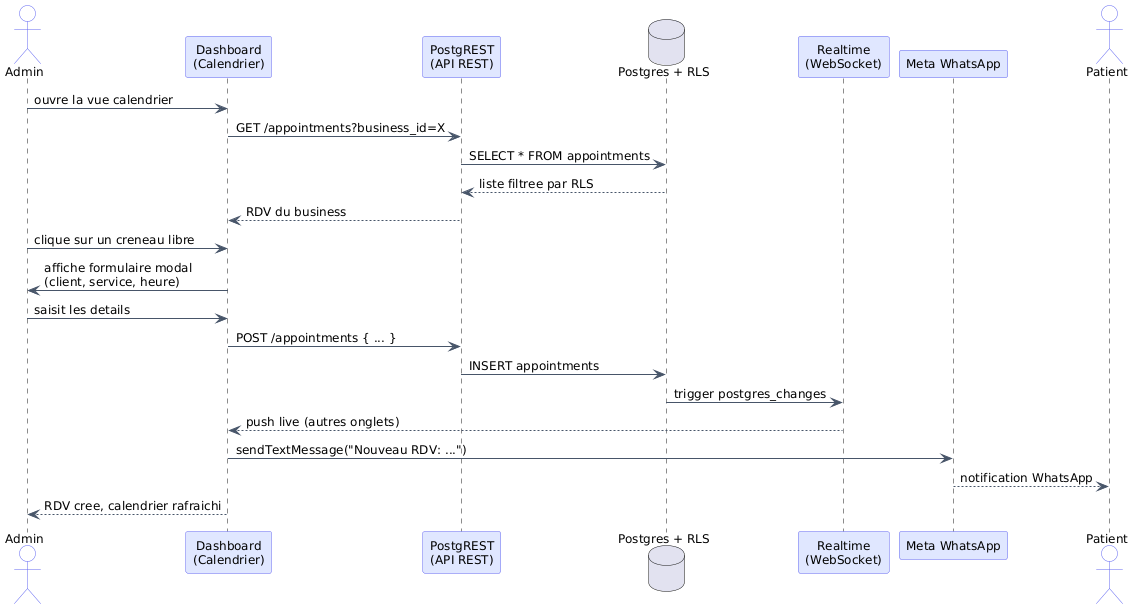
\includegraphics[width=.95\textwidth,height=.6\textheight,keepaspectratio]{figures/seq-s2-rdv.png}%
}{\fbox{\parbox[c][4cm][c]{.85\textwidth}{\centering\itshape\small[seq-s2-rdv.puml -- a generer via plantuml.com]}}}
\caption{Diagramme de séquence : Gérer les rendez-vous (admin via calendrier).}
\label{fig:seq-s2-rdv}
\end{figure}

\paragraph{Consulter dossier médical.}
\begin{figure}[H]\centering
\IfFileExists{figures/seq-s2-dossier.png}{%
  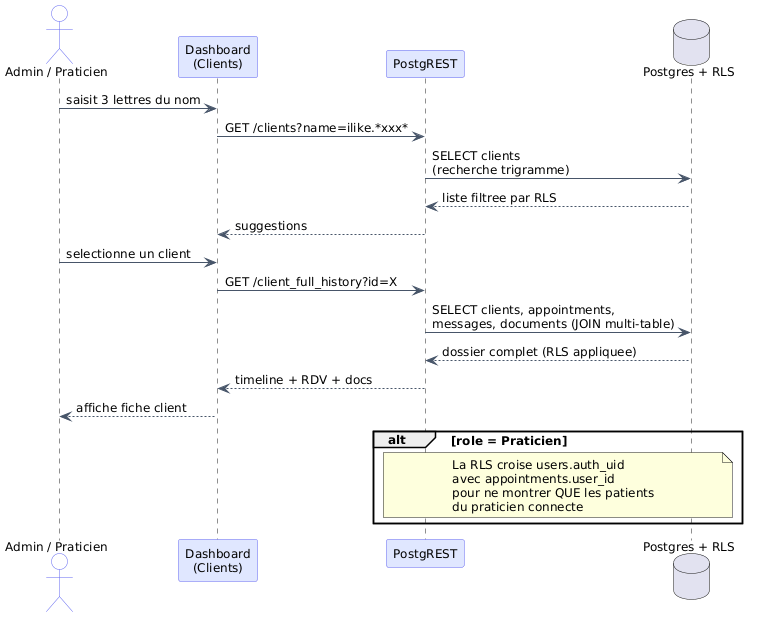
\includegraphics[width=.95\textwidth,height=.55\textheight,keepaspectratio]{figures/seq-s2-dossier.png}%
}{\fbox{\parbox[c][4cm][c]{.85\textwidth}{\centering\itshape\small[seq-s2-dossier.puml -- a generer via plantuml.com]}}}
\caption{Diagramme de séquence : Consulter dossier médical (recherche trigramme + chronologie).}
\label{fig:seq-s2-dossier}
\end{figure}

\paragraph{Envoyer un document (OCR).}
\begin{figure}[H]\centering
\IfFileExists{figures/seq-s2-doc-ocr.png}{%
  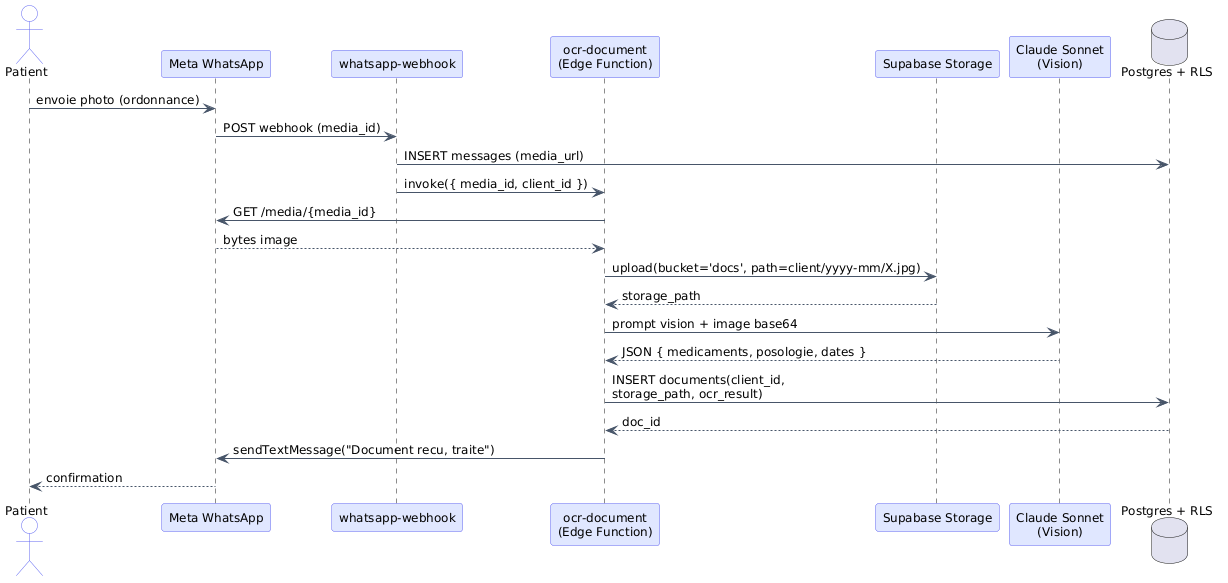
\includegraphics[width=.95\textwidth,height=.6\textheight,keepaspectratio]{figures/seq-s2-doc-ocr.png}%
}{\fbox{\parbox[c][4cm][c]{.85\textwidth}{\centering\itshape\small[seq-s2-doc-ocr.puml -- a generer via plantuml.com]}}}
\caption{Diagramme de séquence : Envoyer un document WhatsApp et extraction OCR par Claude Sonnet.}
\label{fig:seq-s2-doc-ocr}
\end{figure}

\section{Implémentation du Sprint 2}

\subsection{Tableau de bord administrateur}
Le tableau de bord est une \emph{Single Page Application}
monopage. Il s'ouvre sur une vue d'ensemble qui agrège les KPIs
(rendez-vous du jour, taux de \emph{no-shows}, revenus de la
semaine), puis donne accès au calendrier, à la gestion des
rendez-vous et des clients, et aux paramètres.

\begin{figure}[H]\centering
\includegraphics[width=.95\textwidth,keepaspectratio]{figures/dashboard-overview.jpg}
\caption{Tableau de bord administrateur : vue d'ensemble (KPI, derniers rendez-vous).}
\label{fig:dash-overview}
\end{figure}

\begin{figure}[H]\centering
\includegraphics[width=.95\textwidth,keepaspectratio]{figures/dashboard-calendar.jpg}
\caption{Vue calendrier : agenda hebdomadaire filtrable par praticien.}
\label{fig:dash-calendar}
\end{figure}

\begin{figure}[H]\centering
\includegraphics[width=.95\textwidth,keepaspectratio]{figures/dashboard-appointments.jpg}
\caption{Liste des rendez-vous avec filtres de statut.}
\label{fig:dash-appointments}
\end{figure}

\begin{figure}[H]\centering
\includegraphics[width=.95\textwidth,keepaspectratio]{figures/dashboard-clients.jpg}
\caption{Fiche client : historique complet (rendez-vous, messages, documents).}
\label{fig:dash-clients}
\end{figure}

\begin{figure}[H]\centering
\includegraphics[width=.95\textwidth,keepaspectratio]{figures/dashboard-services.jpg}
\caption{Gestion du catalogue de services (nom, durée, prix, catégorie).}
\label{fig:dash-services}
\end{figure}

\subsection{PWA patient}
La PWA partage le même backend Supabase que le tableau de bord,
avec un \emph{service worker} qui met en cache la coquille et les
\emph{assets} pour fonctionner hors ligne. L'onboarding repose
sur un OTP à six chiffres envoyé par WhatsApp via la fonction
\texttt{send-whatsapp-otp}.
\begin{figure}[H]\centering
\includegraphics[width=.55\textwidth,keepaspectratio]{figures/mobile-overview.jpg}
\caption{PWA patient : écran d'accueil après onboarding OTP.}
\label{fig:pwa-overview}
\end{figure}



\begin{figure}[H]\centering
\includegraphics[width=.55\textwidth,keepaspectratio]{figures/mobile-calendar.jpg}
\caption{PWA patient : agenda personnel et prochain rendez-vous.}
\label{fig:pwa-calendar}
\end{figure}

\subsection{Scanner QR patient (check-in PWA)}
Lorsqu'un rendez-vous est confirmé sur WhatsApp, \nova{} envoie au
patient un lien profond qui ouvre une page de check-in dans la PWA.
La figure~\ref{fig:pwa-checkin} montre cet écran~: un QR généré
côté serveur, signé et limité dans le temps, accompagné du nom du
patient, du service réservé, du praticien et de l'horaire. À
l'arrivée à la clinique, l'admin ou le praticien scanne ce QR
depuis le tableau de bord pour démarrer le minuteur de
consultation.

\begin{figure}[H]\centering
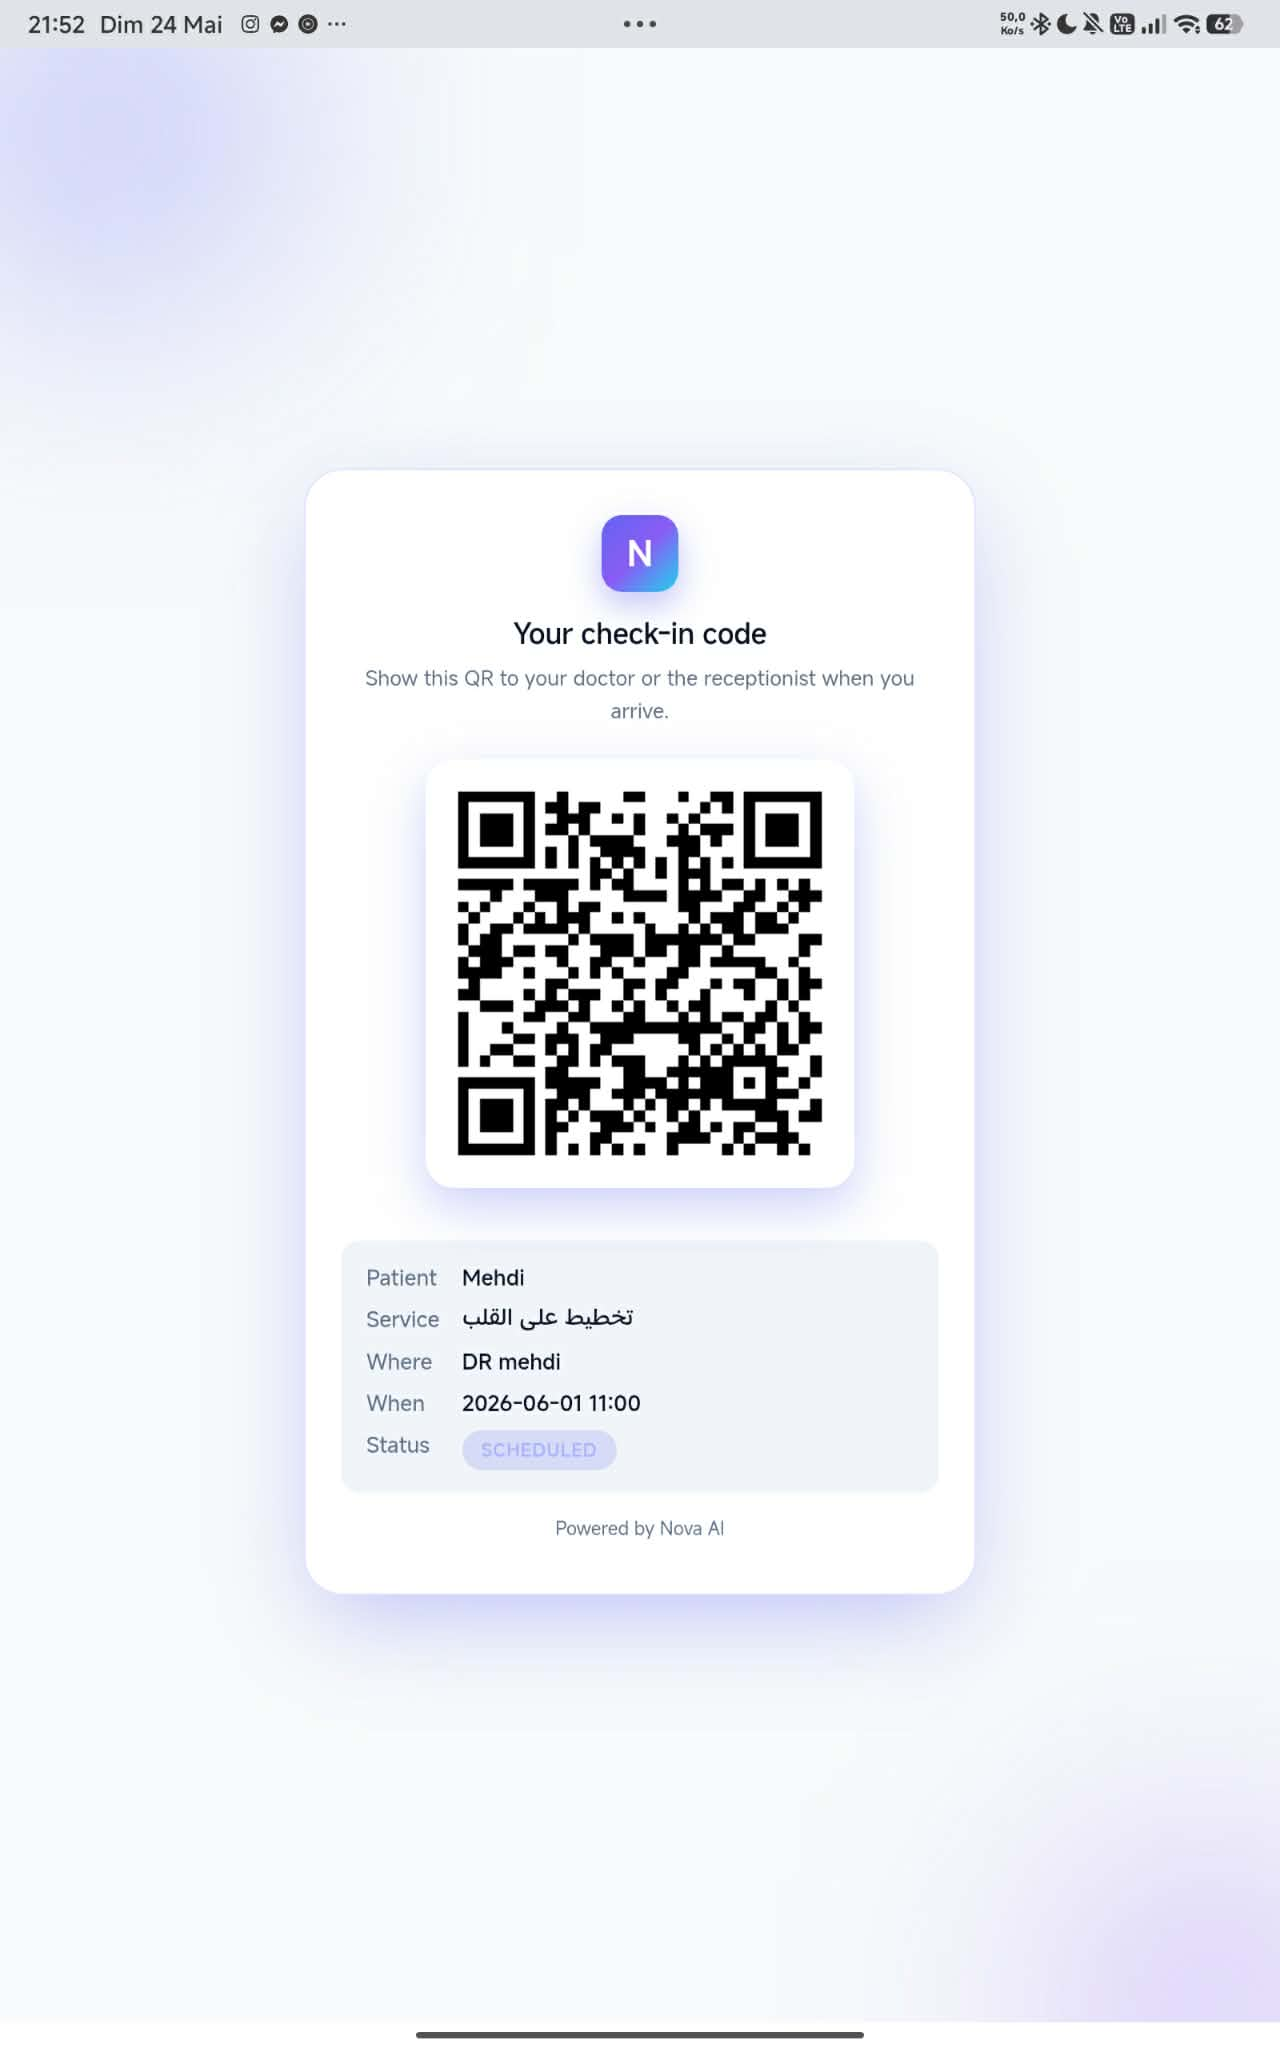
\includegraphics[width=.55\textwidth,keepaspectratio]{figures/pwa-checkin-qr.jpg}
\caption{PWA patient : écran de check-in avec QR signé, informations du rendez-vous et statut.}
\label{fig:pwa-checkin}
\end{figure}



\subsection{OCR de documents WhatsApp}
La fonction Edge \texttt{ocr-document} reçoit l'identifiant d'un
média, le télécharge depuis Meta CDN, le persiste dans Storage,
puis le passe à Claude Sonnet avec un prompt structuré. Le résultat
parsé est attaché au rendez-vous ou directement au dossier patient.
La figure~\ref{fig:wa-ocr} montre un exemple réel~: une ordonnance
manuscrite photographiée par le patient et la liste des analyses
extraites automatiquement par \nova{}, prête à être convertie en
réservation.

\begin{figure}[H]\centering
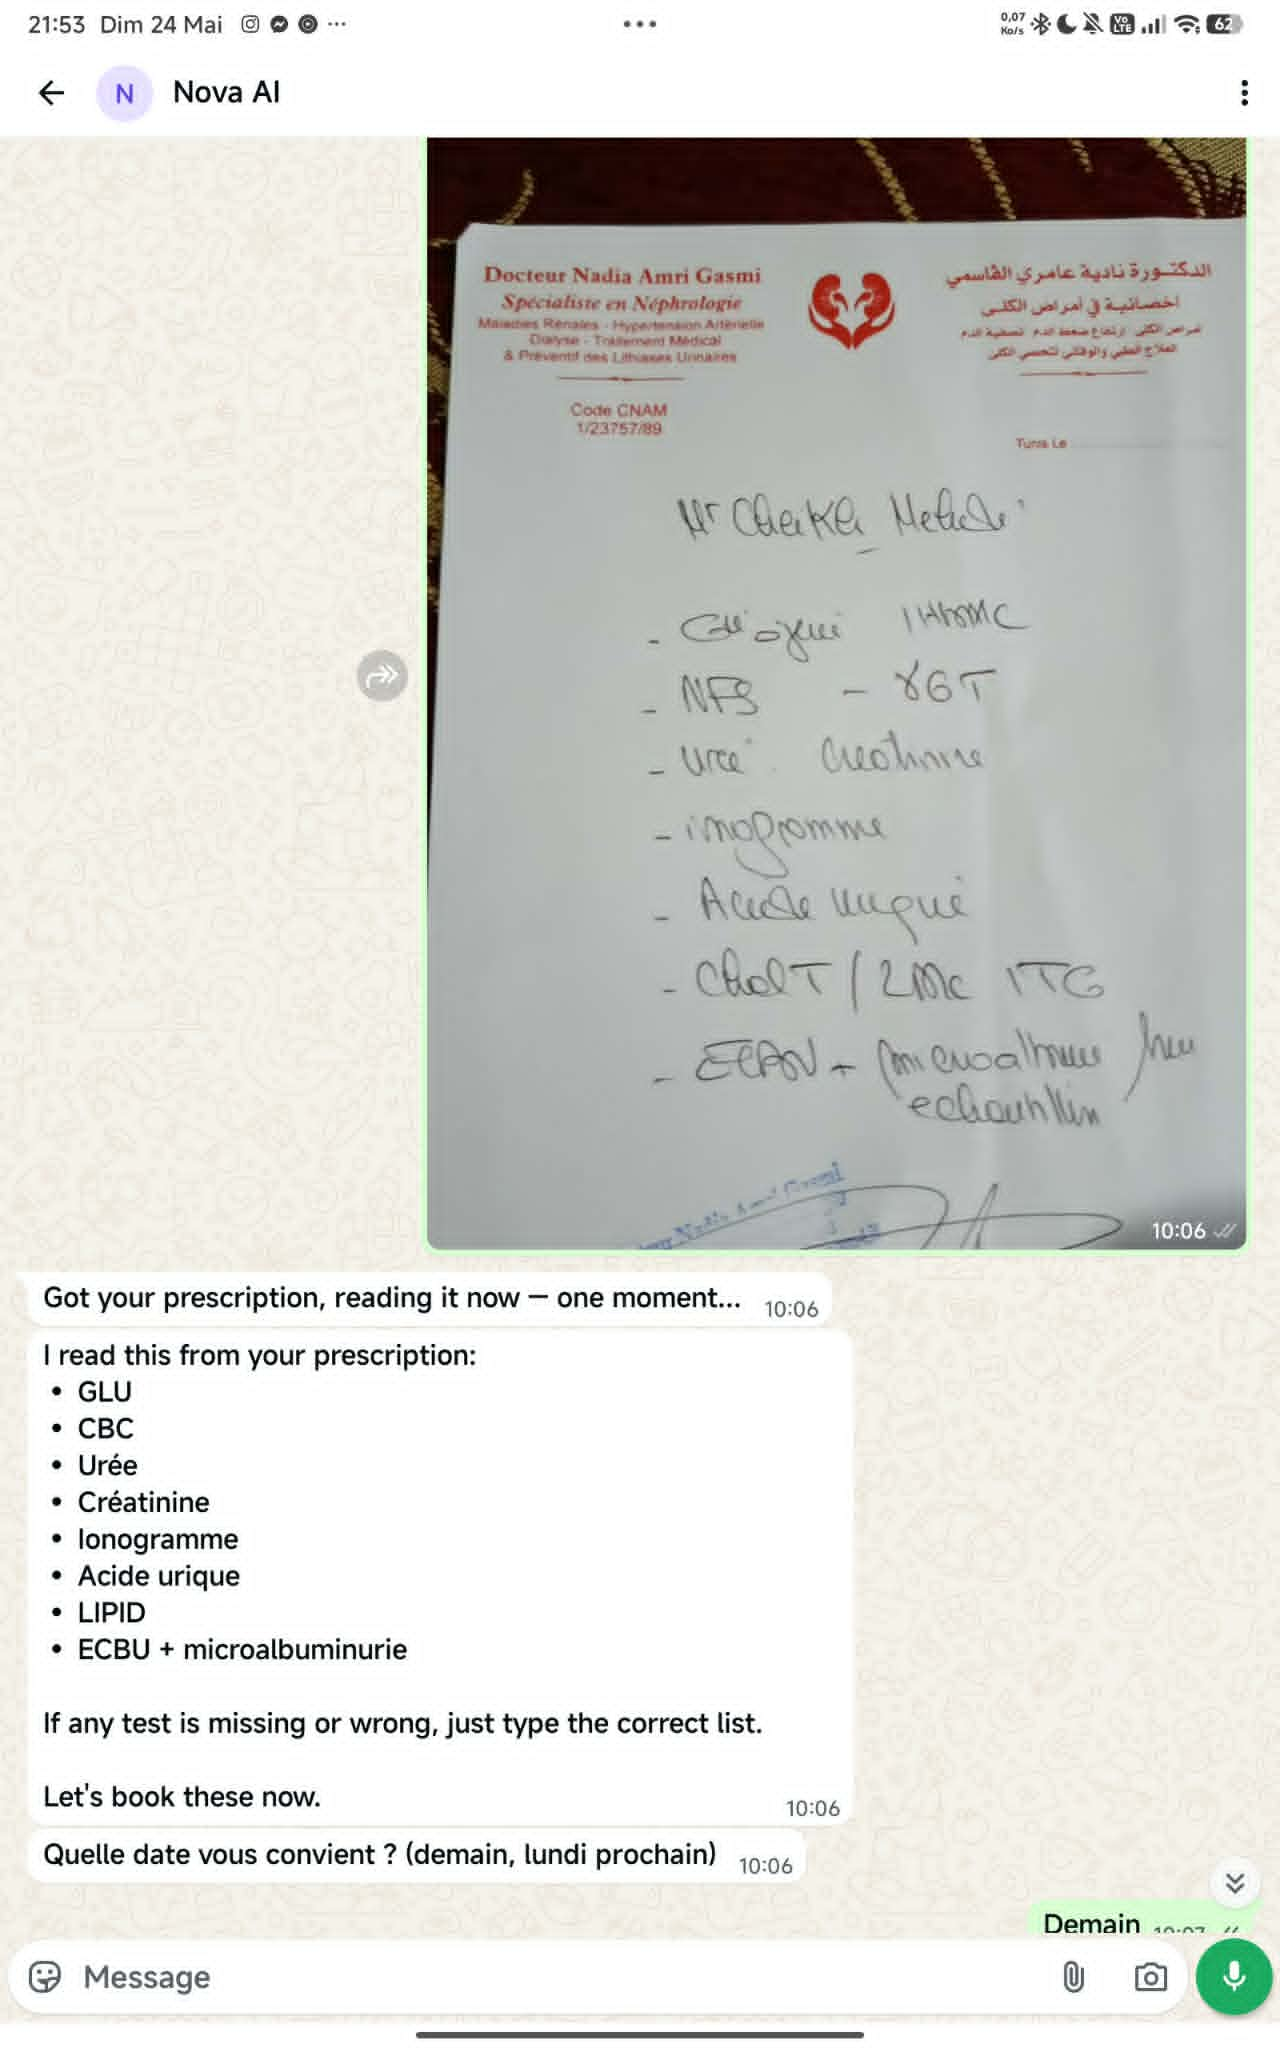
\includegraphics[width=.55\textwidth,keepaspectratio]{figures/whatsapp-ocr-prescription.jpg}
\caption{Conversation WhatsApp : photo d'ordonnance manuscrite, OCR par Claude Sonnet et restitution structurée.}
\label{fig:wa-ocr}
\end{figure}

\section{Tests unitaires et revue du Sprint 2}
\begin{itemize}
  \item \textbf{Calendrier.} Ajouter un rendez-vous via l'IHM,
        vérifier qu'il apparaît en temps réel via Supabase
        Realtime sur un autre onglet ouvert.
  \item \textbf{Recherche client.} Taper trois caractères d'un
        nom, vérifier que la requête trigramme renvoie sous 50~ms.
  \item \textbf{Onboarding PWA.} Envoyer un OTP, vérifier qu'il
        expire après cinq minutes et que le code haché correct
        valide la session.
  \item \textbf{OCR ordonnance.} Envoyer cinq photos types,
        vérifier que les principes actifs sont extraits avec au
        moins 80\,\% de précision.
\end{itemize}

La revue de sprint a validé que l'administrateur peut piloter son
activité depuis une seule interface, que le patient peut consulter
son historique dans la PWA hors ligne, et que les documents envoyés
sur WhatsApp sont automatiquement traités.

\section{Conclusion}
Le Sprint~2 a doté \nova{} des surfaces nécessaires à un usage
quotidien~: tableau de bord opérationnel, PWA patient installable
et OCR de documents. Les fondations du Sprint~1 deviennent ainsi
un produit visible et manipulable. Le Sprint~3 ajoute par-dessus
la couche d'intelligence~: remplissage automatique de créneaux,
apprentissage des durées, vouchers d'anniversaire, packs
sectoriels et assistant vocal.
